% This is samplepaper.tex, a sample chapter demonstrating the
% LLNCS macro package for Springer Computer Science proceedings;
% Version 2.21 of 2022/01/12
%
\documentclass[runningheads]{llncs}
%
\usepackage[T1]{fontenc}
\usepackage{booktabs}
% T1 fonts will be used to generate the final print and online PDFs,
% so please use T1 fonts in your manuscript whenever possible.
% Other font encondings may result in incorrect characters.
%
\usepackage{graphicx}
\usepackage{color}
\usepackage{amsmath}
\usepackage{amssymb}
% Used for displaying a sample figure. If possible, figure files should
% be included in EPS format.
%
% If you use the hyperref package, please uncomment the following two lines
% to display URLs in blue roman font according to Springer's eBook style:
%\usepackage{color}
%\renewcommand\UrlFont{\color{blue}\rmfamily}
%\urlstyle{rm}
%
\begin{document}
%
\title{W2CL:A Multi-Task Learning Approach to Improve Domain-Specific Text Classification through Word Classification and Contrastive Learning}
%
%\titlerunning{Abbreviated paper title}
% If the paper title is too long for the running head, you can set
% an abbreviated paper title here
%
\author{A\inst{1}\orcidID{0000-1111-2222-3333} \and
B\inst{2,3}\orcidID{1111-2222-3333-4444} \and
C\inst{3}\orcidID{2222--3333-4444-5555}}
%
\authorrunning{S. Yan et al.}
\titlerunning{W2CL for Domain Text Classification}
% First names are abbreviated in the running head.
% If there are more than two authors, 'et al.' is used.
%
\institute{Zhejiang Sci-Tech University, Hangzhou, Zhejiang, China\\
\email{email1}\\
\email{\{abc,lncs\}@uni-heidelberg.de}}
%
\maketitle              % typeset the header of the contribution
%
\begin{abstract}
Text classification task plays a crucial role in various NLP tasks. Recent studies have shown that contrastive learning can enhance the representational capability of Pre-trained Language Models(PLMs) and that different methods for constructing positive and negative samples can be applied to various downstream application scenarios. Therefore, in this study, we propose \textbf{W2CL}, a novel multi-task learning framework based on \textbf{W}ord \textbf{C}lassification and \textbf{C}ontrastive \textbf{L}earning, aimed at improving the performance of PLMs in domain-specific text classification task.Contrastive learning assists the model in gradually learning the semantic similarity and contextual relevance between words during the training process to enhance its ability to understand text. Word classification provides additional contextual understanding, thereby improving the model's ability to differentiate between different classes within the specific domain. Experiments demonstrate that our multi-task approach significantly outperforms other methods, leading to substantial improvements in domain-specific text classification performance. This framework offers a robust solution for adapting general-purpose language models to specialized domains, ensuring higher accuracy and better generalization in various practical applications.

\keywords{Text Classification  \and Contrastive Learning \and Multi-task Learning.}
\end{abstract}
%
%
%
\section{Introdction}
\label{sec:intro}
In recent years, mainstream text classification tasks have largely relied on deep representation learning methods, especially PLMs such as BERT\cite{bert}, RoBERTa\cite{roberta}, and T5\cite{t5}. Although the vector representations from these models capture richer textual features compared to traditional methods, simple fine-tuning is insufficient for integrating domain-specific knowledge into language models for domain-specific text classification. Therefore, we propose the W2CL framework to effectively incorporate domain knowledge into the language model.

With the development of large language models(LLMs)\cite{bert,lm5,lm1,roberta,lm6,lm2,lm4,lm3}, particularly ChatGPT\cite{gpt}, which has attracted significant attention from NLP researchers, some studies\cite{gptuse2,gptuse1,gptuse5,gptuse4,gptuse3} have shown that ChatGPT has demonstrated impressive performance, outperforming many models even in zero-shot settings. Therefore, we leverage the powerful capabilities of ChatGPT to generate the necessary domain knowledge for our W2CL framework, such as domain-specific vocabulary and word classifications.

Meanwhile, numerous studies have demonstrated that integrating effective knowledge with PLMs can enhance the performance of these models on certain downstream tasks.LIBERT\cite{libert} adds a lexical relationship classification task to the original BERT pre-training tasks to help the model acquire richer semantic information. SenseBERT\cite{sensebert} adds a part-of-speech layer to the BERT model, that is, it adds part-of-speech information of words (such as noun.food and noun.state, etc.) to the original input, and uses the representation vector after integrating part-of-speech information for masking tasks and part-of-speech classification tasks.SKEP\cite{skep} integrates sentiment knowledge (sentiment words, sentiment polarity, and aspect-sentiment pairs) into the model by designing three types of sentiment analysis tasks. Sentiprompt\cite{sentiprompt} integrates sentiment knowledge by constructing different paradigm templates and masking aspects, polarities, and opinions in the templates, and designing tasks to predict the masked tokens. LET\cite{let} integrates all classification definitions of HowNet entities into the input, uses the original input and classification information for masking tasks, and finally integrates the knowledge contained in HowNet into the model. KEAR\cite{kear} directly faces the multiple-choice task, integrates the knowledge relationship of questions and options, the dictionary’s definition knowledge of questions and options, and the knowledge of annotated training samples into the model, improving the model’s performance in the commonsense knowledge question answering task.

The aforementioned methods combine knowledge with pre-training tasks to enhance the performance of models in various downstream tasks. However, these methods have two issues: First, the form of knowledge is fixed and difficult to acquire; Second, in order to utilize the knowledge, new neural network layers need to be designed, which increases the training cost.

For issue 1, we utilize ChatGPT to acquire domain knowledge, a process that is both simple and results in high-quality knowledge. For issue 2, we employ the W2CL framework to integrate this domain knowledge, which requires only the addition of a classification layer, thereby consuming minimal computational resources.

In the field of NLP, recent popular contrastive learning methods typically construct positive and negative samples at the sentence level. SimCSE\cite{simcse} uses the randomness of the dropout layer to construct positive samples, treating other samples in the same batch as negative samples. The training objective is to minimize the vector distance between the positive samples and the current sample, while maximizing the vector distance between the negative samples and the current sample.Building on SimCSE, ESimCSE\cite{esimcse} uses the principle that word repetition generally does not change the meaning of a sentence to construct positive samples.PromptBERT\cite{promptbert} applies multiple templates that do not affect semantics within the same sample, treating samples reconstructed with different templates as positive samples.BGE\cite{bge} directly targets downstream paragraph retrieval tasks, treating the question and its corresponding answer as positive samples, and other samples in the same batch as negative samples. It has shown excellent performance in Chinese paragraph retrieval tasks.For domain-specific tasks, domain vocabulary contains more domain-specific information compared to sentences, and domain knowledge is easier to construct. However, the aforementioned contrastive learning methods are all based on sentences. Therefore, we propose a word-level contrastive learning method and also introduce a word classification task to provide additional contextual understanding, further boosting the model's performance in domain tasks.

Our contributions can be summarized from three perspectives. 1) We propose a novel framework called W2CL, which can better transfer general models to specific domains. 2) We propose a novel and simple general method for knowledge extraction and integration. The knowledge extraction method based on ChatGPT and the knowledge integration method based on word-level contrastive learning and word classification are both effective and scalable. 3) Our experimental results demonstrate that the proposed method can enhance the performance of various language models across multiple domains and tasks, indicating that the W2CL framework is both effective and generalizable.



\section{The Proposed Method}
\label{sec:method}
This section introduces the detailed methodology of the our proposed W2CL framework, which mainly consists of two parts: domain knowledge extraction with ChatGPT and knowledge integration based on multi-task learning.
\subsection{Domain Knowledge Extraction with ChatGPT}
In the domain knowledge acquisition phase, we use ChatGPT as a knowledge extractor to extract the necessary domain knowledge for multi-task learning from raw text corporas which can be easily obtained from online resources like Baidu Zhidao. This step can be divided into three stages, as shown in Figure~\ref{ke}.

In Step 1, we first use the Jieba tool to segment the raw text corpus and then compile a list of frequently occurring words. ChatGPT is then employed to filter out domain-specific vocabulary from this list, as illustrated in Figure~\ref{ke}.a, and the prompt1 shown in the Figure~\ref{ke} is "I currently have several terms. You will categorize all the terms I provide into levels of relevance: high, medium, and low. This relevance level pertains to the XX domain". Finally, extract the terms with high relevance to compile the final domain-specific vocabulary list.

In Step 2, ChatGPT is used to categorize the domain-specific vocabulary obtained in Step 1 into relevant categories within the domain, and the prompt2 is "Assume you are now an expert in the XX domain. Please classify the terms I provide within the subcategories of this domain.". This step allows us to obtain the initial version of domain-specific classification knowledge.

In Step 3, we manually consolidate all categories obtained in Step 2 to create a final comprehensive category list that covers all terms. Finally, we provide ChatGPT with this finalized category list to reclassify the vocabulary, producing the ultimate domain knowledge, and the prompt3 is "Assume you are an expert in the XX domain. I will provide you with several terms related to this domain, along with a list of categories: [Categories]. I need you to assign each of my terms to a category from the provided list. If a term cannot be assigned to any of the existing categories, please mark it as None. The required format for the response is 'Term: Category'.".

\begin{figure}[ht]
	\centering
	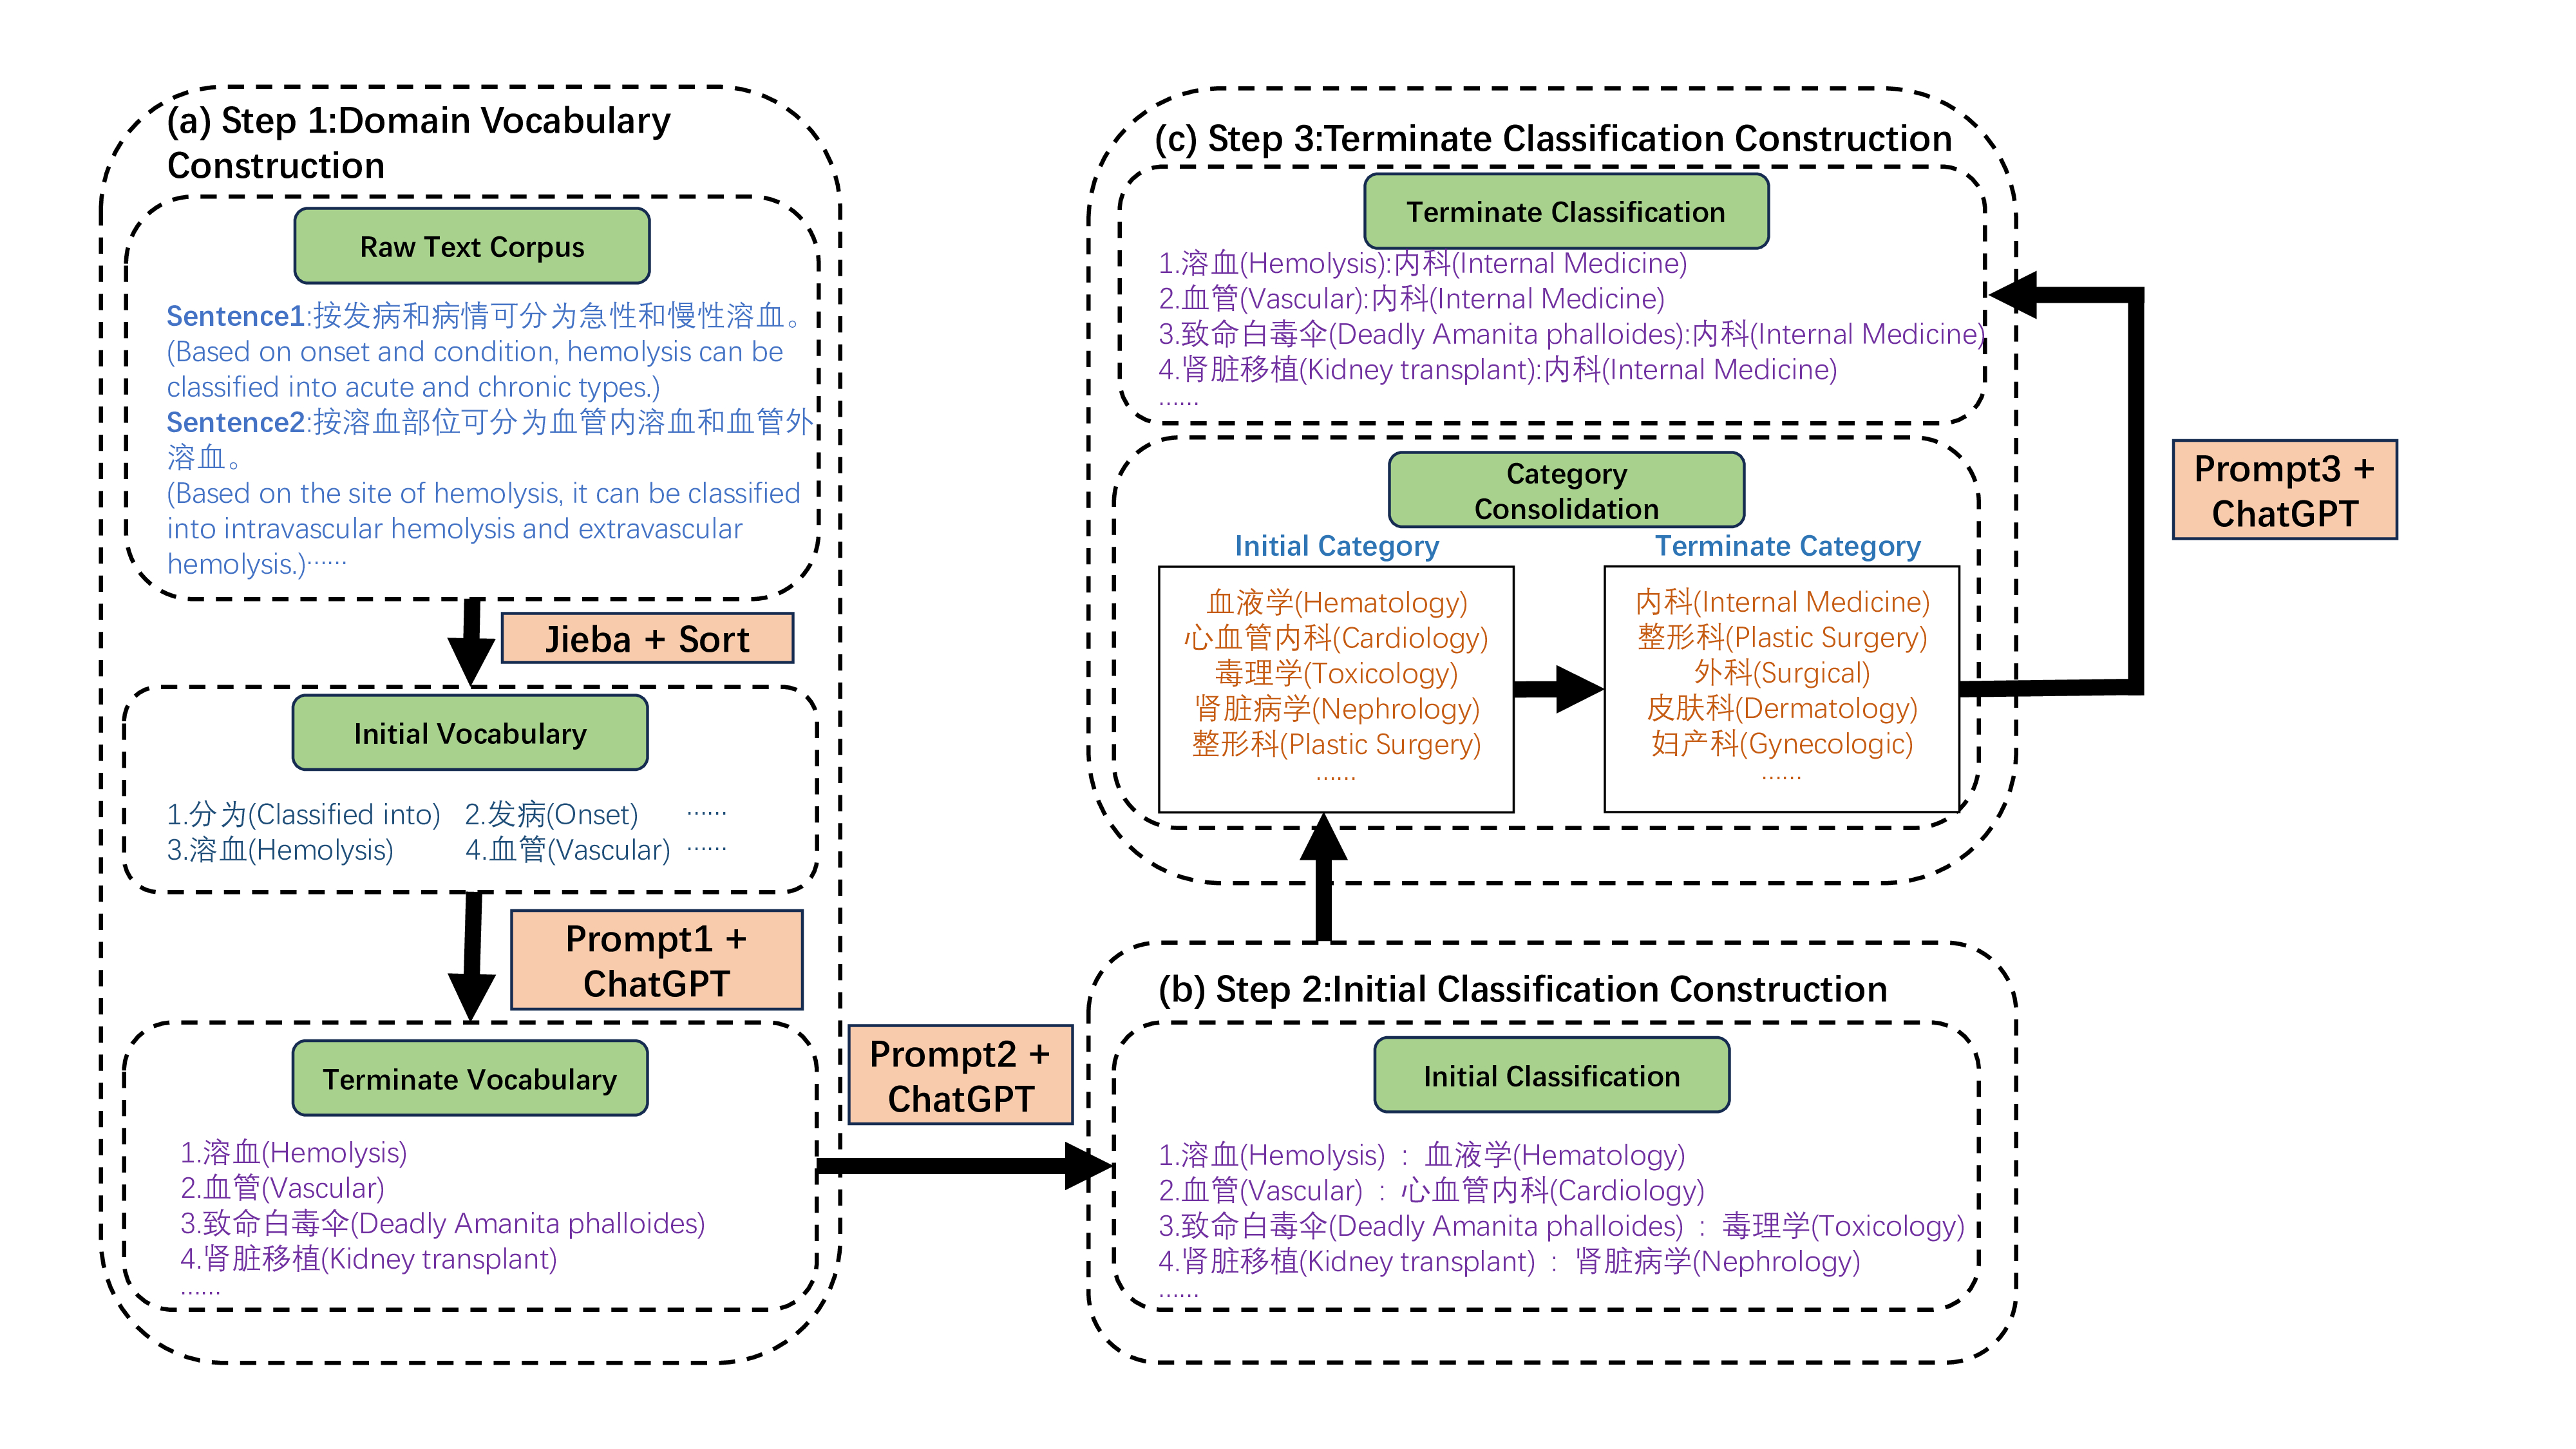
\includegraphics[width=1.0\textwidth]{ChatGPT} 
	\caption{Knowledge Extraction Framework}
	\label{ke}
\end{figure}
\subsection{Domain Knowledge Integration}
Our proposed knowledge integration method is based on Whole Word Masking(WWM)\cite{macbert} and incorporates two additional training tasks: Word Classification and Contrastive Learning. The details about WWM will be introduced in the BASELINES section of Chapter 3. The following sections will introduce other two tasks individually.
\subsubsection{Word Classification.}
Given a sentence \{$x${\tiny 1}, $x${\tiny 2}, $x${\tiny 3}, [MASK], $x${\tiny 5}, [MASK],$x${\tiny 7}\} where \($x$_i\) means one word which may cover several tokens and a list of categories for the masked words \{$C${\tiny 1}, $C${\tiny 2}\}. Word Classification adds a classification layer to the original model architecture. The classification loss function is then computed as shown in Equation~\ref{tc}:
\begin{equation}
	\label{tc}
	L(\mathbf{y}, \mathbf{\hat{y}}) = - \sum_{i=1}^C \left( y_i \log(\hat{y}_i) + (1 - y_i) \log(1 - \hat{y}_i) \right)
\end{equation}
\begin{itemize}
	\item $\mathbf{y} = [y_1, y_2, \ldots, y_C]$: The multi-label binary vector of true labels, where $C$ is the number of classes. Each $y_i$ represents the true label for class $i$ ($1$ indicates the presence of the class, $0$ indicates the absence of the class).
	\item $\mathbf{\hat{y}} = [\hat{y}_1, \hat{y}_2, \ldots, \hat{y}_C]$: The predicted probability distribution vector from the model, where each $\hat{y}_i$ represents the predicted probability for class $i$, with values in the range $[0, 1]$.
	\item $L(\mathbf{y}, \mathbf{\hat{y}})$: The loss function value for the multi-label classification task.
\end{itemize}
\subsubsection{Contrastive Learning.}
Given a sentence \{$x${\tiny 1}, $x${\tiny 2}, $x${\tiny 3}, [MASK], $x${\tiny 5}, [MASK],$x${\tiny 7}\} where \($x$_i\) means one word which may cover several tokens, and the actual words masked by [MASK] \{$x${\tiny 4}, $x${\tiny 6}\}. Our proposed contrastive learning method uses the actual word corresponding to the current [MASK] position as the positive sample for the current [MASK]. All the positive samples of other [MASK] tokens from other sentences in the same batch are used as the negative samples for the current [MASK]. The specific calculation method is shown in Equation~\ref{cl}:
\begin{equation}
	\label{cl}
	L(\mathbf{t}, \mathbf{t'}) = -\frac{1}{N} \sum_{i=1}^{N} \log \frac{e^{sim(f(\mathbf{t}_i) \cdot f(\mathbf{t'}_i))/\tau}}{\sum_{j=1}^{N} e^{sim(f(\mathbf{t}_i) \cdot f(\mathbf{t'}_j))/\tau}}
\end{equation}
\begin{itemize}
	\item $\mathbf{t} = [t_1, t_2, \ldots, t_N]$: $N$ is the number of [MASK] in one batch. Each $f$($t_i$) represents the representation of $i_{st}$ [MASK] token in the batch.
	\item $\mathbf{t'} = [t'_1, t'_2, \ldots, t'_N]$: $f$($t'_i$) represents the representation of the true label $t'_i$ corresponding to the $i_{st}$ [MASK] token, which is the positive sample for $f$($t_i$).
	\item $L(\mathbf{t}, \mathbf{t'})$: The loss function value for the contrastive learning task.
	\item \(sim(\mathbf{h1} \cdot \mathbf{h2})\): \(sim(\mathbf{h1} \cdot \mathbf{h2})\) is the cosine similarity \(\tfrac{\mathbf{h1}^T\mathbf{h2}}{\lVert \mathbf{h1} \rVert \cdot \lVert \mathbf{h2} \rVert}\).
	\item \(\tau\): is a temperature hyperparameter, with a default value of 0.01.
\end{itemize}
\subsubsection{Training Framework.}
The overall training objective comprises three parts:
\begin{equation}
	\label{allloss}
	L_{overall} = L_{WWM} + L_{WC} + L_{CL} 
\end{equation}
where \(L_{WWM}\) is the loss of the WWM task, \(L_{WC}\) is calculated by equation~\ref{tc}, and \(L_{CL}\) is calculated by equation~\ref{cl}.

\begin{figure}[ht]
	\centering
	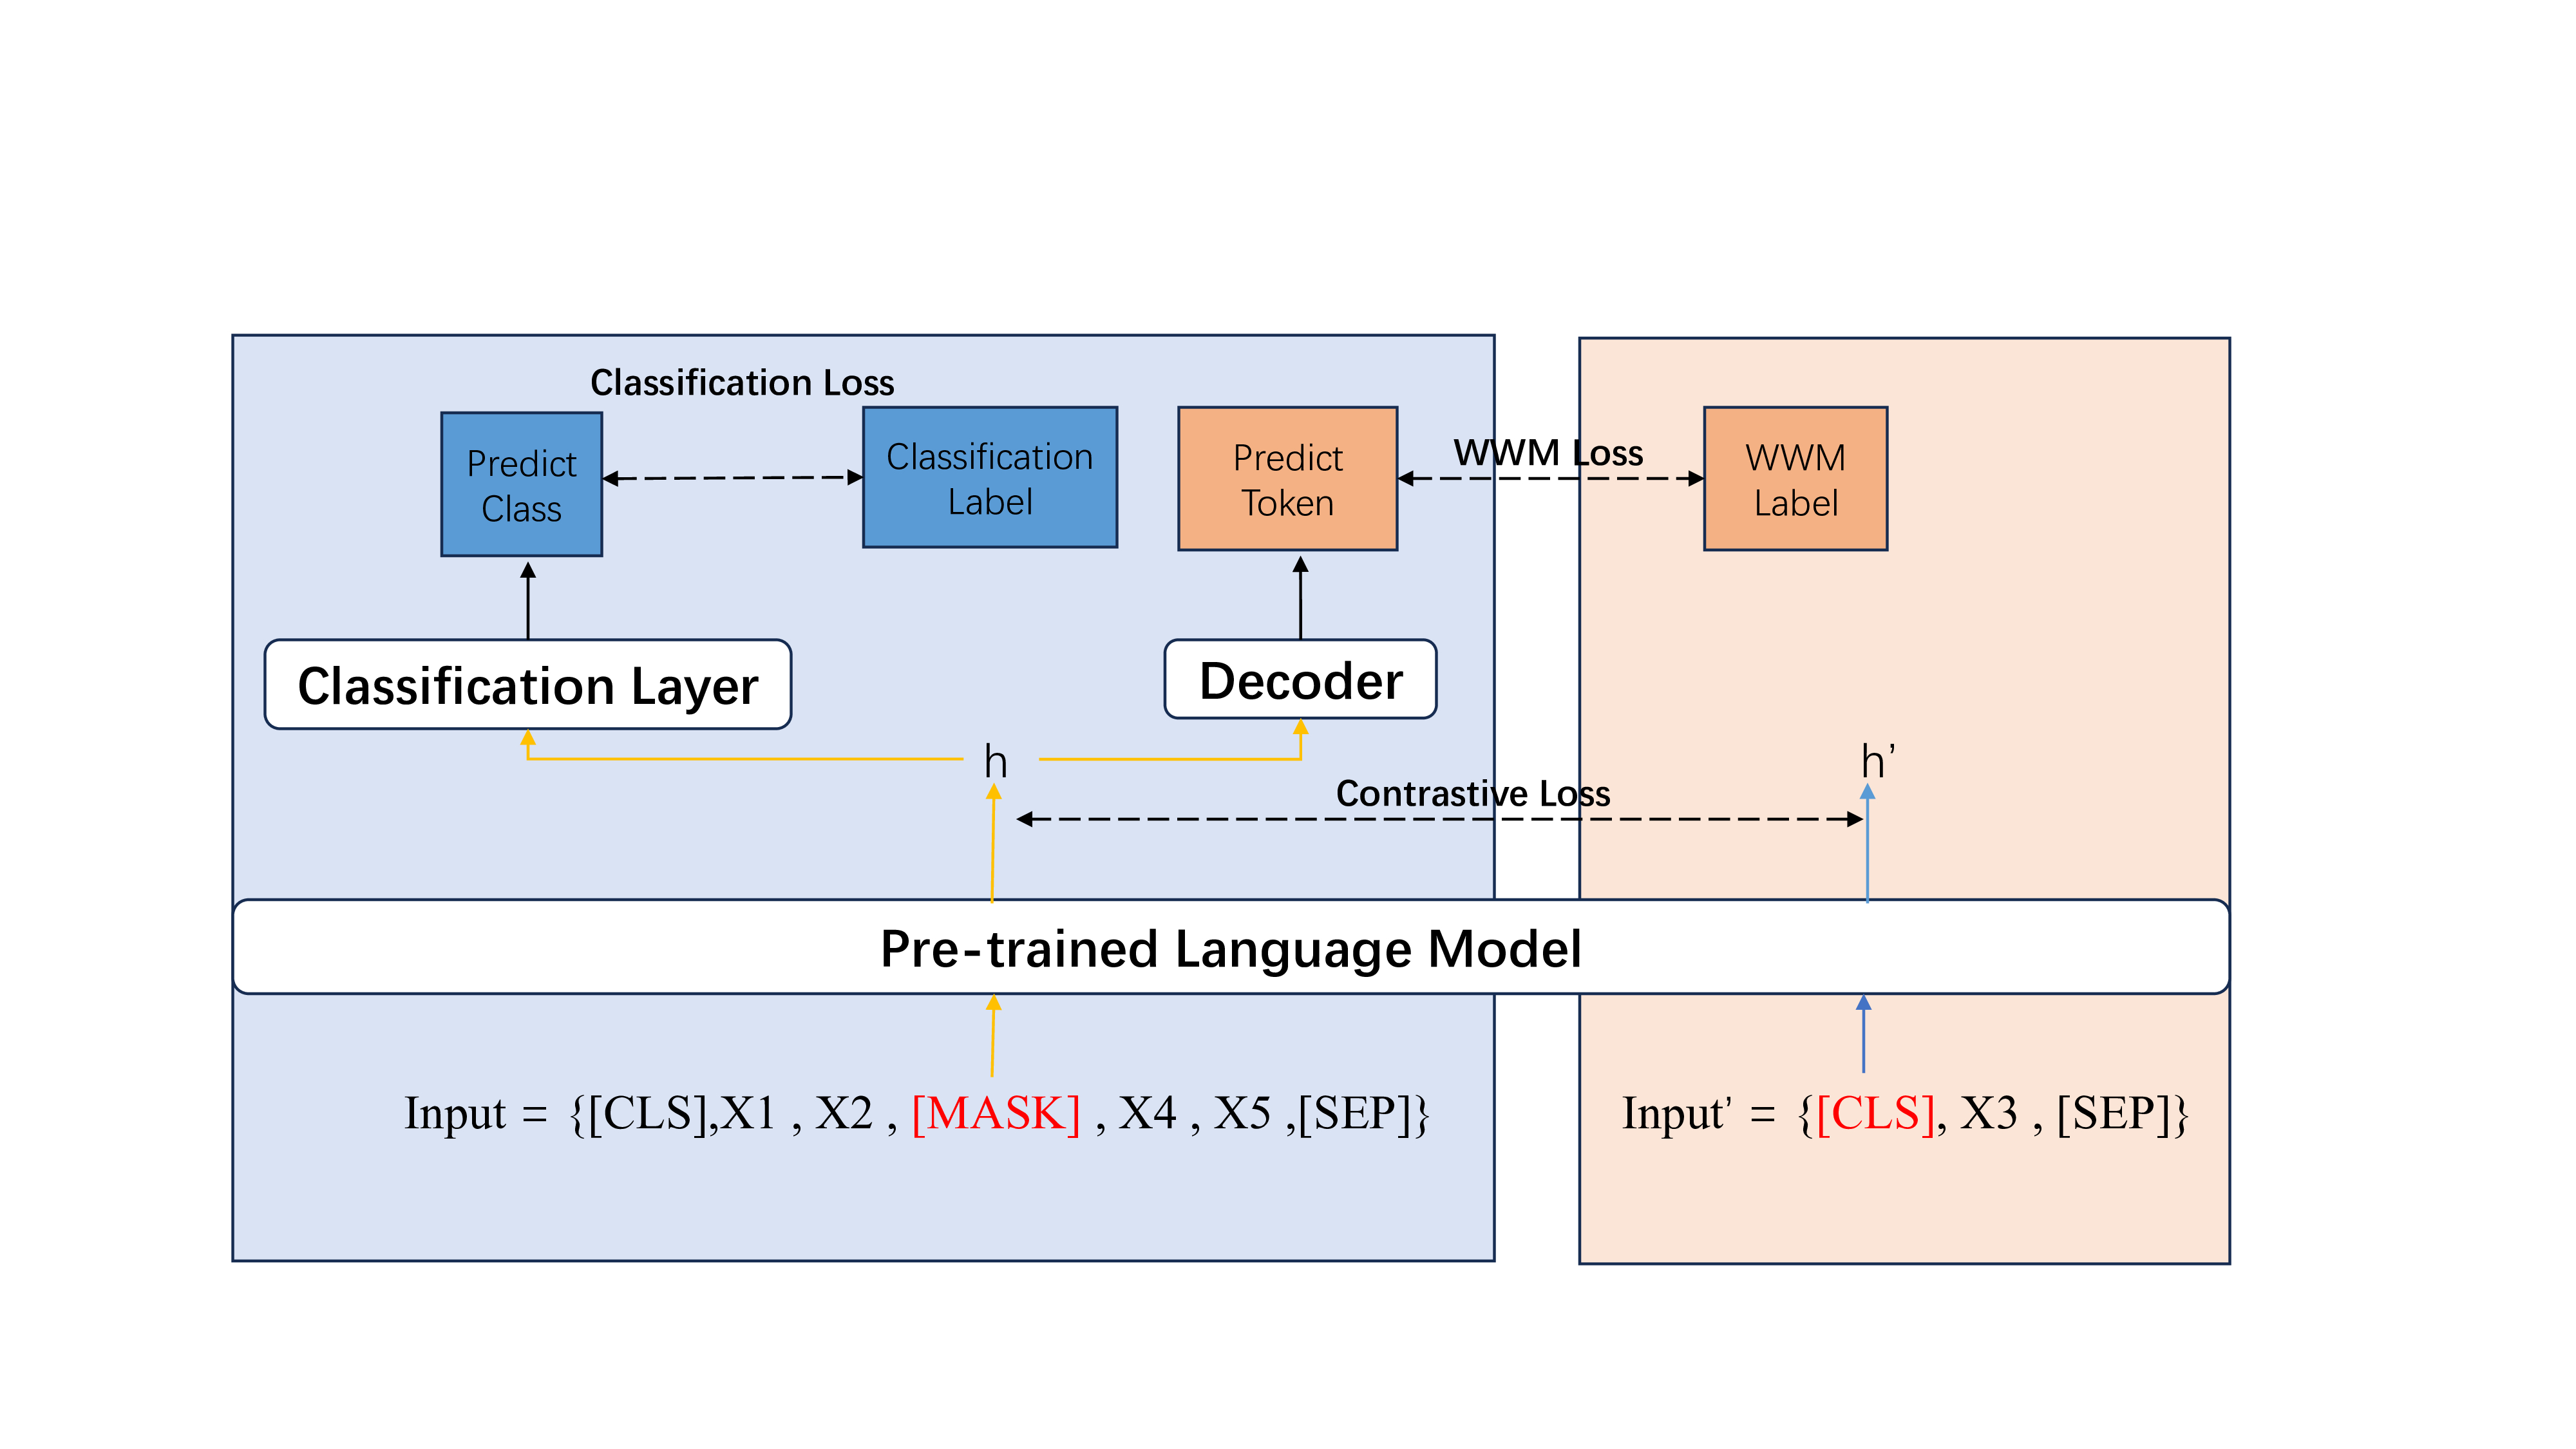
\includegraphics[width=1.0\textwidth]{train_framework} 
	\caption{Training Framework}
	\label{train}
\end{figure}

The training framework is depicted in Figure~\ref{train}. Firstly, we obtain the loss(\(L_{WWM}\)) for the WWM task, which aims to help the model learn the meanings, usage, and contextual relationships of vocabulary, facilitating the model's adaptation to the specific domain context. Secondly, the loss(\(L_{CL}\)) from contrastive learning can assist the model in gradually learning the semantic similarity and contextual relevance between words during the training process, thereby enhancing its ability to understand text. Finally, the loss(\(L_{WC}\)) from word classification provides additional contextual understanding and domain knowledge, thereby improving the model's ability to differentiate between different classes within the specific domain.



\section{Experiments}
\label{sec:exp}
In this chapter, we validate the proposed W2CL method on sentence classification tasks across four domains. Additionally, we demonstrate the effectiveness of this method in domain transfer tasks.
\subsection{Dataset and Experiment Details}
We evaluated the proposed multi-task learning method on four sentence classification datasets, covering the domains of automotive, legal, finance, and medicine. For the transfer learning tasks, we assessed the method on four text retrieval datasets from the same domains. For the sentence classification task datasets, the automotive and financial domains are the datasets we contributed, while the legal and medical domains use public datasets. The text retrieval task datasets are all contributed by us. Below, we provide a brief introduction to these datasets.

\subsubsection{Sentence Classification Dataset.} The evaluation sets for sentence classification task consist of four datasets: Automatic Sentence Classification Corpora (ASCC), CAIL~\cite{cail}, CHIP-CTC~\cite{chip}, and Finance Sentence Classification Corpora (FSCC). ASCC pertains to the automotive domain and includes 6174 training instances and 1000 test instances, with coverage of 10 categories. CAIL is related to the legal domain and comprises 154592 training instances and 49639 test instances, encompassing 134 categories. CHIP-CTC pertains to the medical domain, with 24516 training instances and 6128 test instances, covering 44 categories. FSCC is a finance-related dataset, consisting of 10346 training instances and 3332 test instances, and spans 14 categories.

\subsubsection{Text Retrieval Dataset.} The text retrieval datasets comprise four collections: Automatic Text Retrieval Corpora (ATRC), Legal Text Retrieval Corpora (LTRC), Medical Text Retrieval Corpora (MTRC), and Finance Text Retrieval Corpora (FTRC). These datasets correspond to the automotive, legal, medical, and financial domains, respectively. Each dataset contains 1000, 232, 3520, and 1953 retrieval test texts, with a retrieval text space of 7175, 5232, 15000, and 12000 texts accordingly.

\subsubsection{Experiment Details.} Our model begins with the checkpoint of BERT/RoBERTa model, and we utilize the [CLS] token representation as the sentence representation. During training, we employe an Adam optimizer with a batch size of 16. The learning rate for the sentence representation model is set to 5e-5. During the fine-tuning stage, we modified the learning rate to 3e-5 based on the training hyperparameters. Additionally, we set the seed to 0, 1, and 2, respectively, and calculated the average experimental data metrics for these three scenarios.

\subsection{BASELINES}
We validated the effectiveness of our proposed method by comparing it against three baseline approaches: Whole Word Masking(WWM), SimCSE, and SSCL\cite{sscl}, using BERT and RoBERTa as basic models.

\subsubsection{WWM.} WWM modifies the random masking task by changing the masking unit from token to whole word, leveraging contextual information to predict the masked word. For instance, in WWM, both "play" and "\#ing" would be masked together. We selected WWM as a baseline method instead of random masking because, for domain-specific tasks, domain-specific word tends to contain more domain-relevant information.

\subsubsection{SimCSE.} SimCSE constructs positive samples based on the randomness of dropout and uses in-batch sampling to create negative samples. The model is trained by generating a loss value through the contrast between the original samples and the positive and negative samples.

\subsubsection{SSCL.} SSCL enhances the construction of negative samples by leveraging the principles of SimCSE. Specifically, SSCL employs hidden representations from intermediate layers of PLMs as negative samples. The objective is to ensure that the final sentence representations are distinctly separated from these intermediate representations.

\subsection{Experiment Results}
In this chapter, we will present the experimental results for the sentence classification and retrieval tasks. F1 score and Mean Reciprocal Rank(MRR) are used as evaluation metrics for these two tasks, respectively. 
\subsubsection{Sentence Classification Task.}Table~\ref{f1_tab} presents the performance of various methods on the sentence classification task, with F1 score as the evaluation metric. From the experimental results, it can be observed that the proposed W2CL method outperforms other methods. Compared to the WWM method, W2CL incorporates contrastive learning task and word classification task on top of WWM. In comparison to SimCSE and SSCL methods, W2CL modifies the construction of positive and negative samples for contrastive learning and introduces word classification task. Based on the experimental results, the following conclusions can be drawn: 1) Domain knowledge constructed based on ChatGPT is effective; 2) The proposed W2CL method effectively integrates domain knowledge into the model; 3) The proposed W2CL method outperforms other methods across different baseline models and domains. This indicates that W2CL can serve as a universal method, adaptable to any model as the basic model and transferable across various domains.

\begin{table}
	\caption{ Evaluation performance on the sentence classification tasks. The evaluation metric is F1 score(\%).}\label{f1_tab}
	\begin{center}
	\begin{tabular}{lcccll}
		\bottomrule
		Model          & ASCC  & CAIL  & CHIP-CTC & \multicolumn{1}{c}{FSCC} & \multicolumn{1}{c}{Avg.} \\ \hline
		\multicolumn{6}{c}{\textit{BERT Version}}                                                                \\ \hline
		BERT           & ~~~92.48~~~ & ~~~65.58~~~ & ~~~82.91~~~    & ~~~85.82~~~                    &         ~~~81.70~~~                 \\ \hline
		WWM-BERT       & ~~~94.08~~~ & ~~~66.62~~~ & ~~~83.52~~~    & ~~~85.91~~~                    &         ~~~82.53~~~               \\ \hline
		SimCSE-BERT    & ~~~93.70~~~  & ~~~66.68~~~ & ~~~83.64~~~    & ~~~85.81~~~                    &        ~~~82.46~~~                 \\ \hline
		SSCL-BERT      & ~~~93.76~~~ & ~~~66.43~~~ & ~~~83.56~~~    & ~~~85.67~~~                    &         ~~~82.36~~~                 \\ \hline
		W2CL-BERT(Ours)       & ~~~\textbf{94.93}~~~ & ~~~\textbf{66.83}~~~ & ~~~\textbf{84.06}~~~    & ~~~\textbf{86.08}~~~                    &             ~~~\textbf{82.98}~~~             \\ \hline
		\multicolumn{6}{c}{\textit{RoBERTa Version}}                                                             \\ \hline
		RoBERTa        & ~~~93.93~~~ & ~~~67.38~~~ & ~~~83.91~~~    & ~~~86.10~~~                     &        ~~~82.83~~~                  \\ \hline
		WWM-RoBERTa    & ~~~94.26~~~ & ~~~67.46~~~ & ~~~83.59~~~    & ~~~86.11~~~                    &       ~~~82.86~~~                  \\ \hline
		SimCSE-RoBERTa & ~~~94.14~~~ & ~~~67.43~~~ & ~~~83.92~~~    & ~~~85.83~~~                    &        ~~~82.83~~~                  \\ \hline
		SSCL-RoBERTa   & ~~~94.41~~~ & ~~~67.18~~~ & ~~~83.56~~~    & ~~~86.27~~~                    &        ~~~82.86~~~                  \\ \hline
		W2CL-RoBERTa(Ours)     & ~~~\textbf{94.84}~~~ & ~~~\textbf{67.71}~~~ & ~~~\textbf{83.98}~~~    & ~~~\textbf{86.53}~~~                    &          ~~~\textbf{83.27}~~~                \\ \bottomrule
	\end{tabular}
	\end{center}
\end{table}


\subsubsection{Transfer Task.}In this section, we evaluate the generalization ability of the proposed W2CL method on text retrieval tasks across four domains. The objective of this task is to rank the candidate retrieval texts based on their similarity to the given retrieval text. For this task, we directly utilize the representation vector of the [CLS] token, without the need for fine-tuning.

The experimental results are shown in Table~\ref{mrr_tab}. From the table, it can be observed that the proposed W2CL method achieves superior MRR scores on most datasets. This result indicates that the W2CL method exhibits better generalization ability compared to other methods in the study. When using RoBERTa as the basic model, the average MRR of WWM and SimCSE is lower than that of RoBERTa. As shown in the table, this is mainly because the MRR of WWM and SimCSE is lower than RoBERTa on the automotive domain dataset, leading to a lower average MRR. Since there is no fine-tuning phase in this task, we guess that this is primarily due to the randomness of the dataset and pre-training.

\begin{table}[]
	\caption{ Evaluation performance on the text retrieval tasks. The evaluation metric is MRR score(\%).}\label{mrr_tab}
	\begin{center}
	\begin{tabular}{lcccll}
		\bottomrule
		Model          & ATRC  & LTRC  & MTRC  & \multicolumn{1}{c}{FTRC} & \multicolumn{1}{c}{Avg.} \\ \hline
		\multicolumn{6}{c}{\textit{BERT Version}}                                                             \\ \hline
		BERT           & ~~~5.22~~~  & ~~~63.36~~~ & ~~~53.86~~~ & ~~~48.91~~~                    &     ~~~42.84~~~                     \\ \hline
		WWM-BERT       & ~~~63.33~~~ & ~~~76.93~~~ & ~~~78.14~~~ & ~~~62.81~~~                    &     ~~~70.30~~~                     \\ \hline
		SimCSE-BERT    & ~~~68.48~~~ & ~~~84.49~~~ & ~~~86.90~~~ & ~~~66.48~~~                    &     ~~~76.59~~~                     \\ \hline
		SSCL-BERT      & ~~~32.91~~~ & ~~~85.85~~~ & ~~~79.70~~~ & ~~~79.44~~~                    &     ~~~69.48~~~                     \\ \hline
		W2CL-BERT(Ours)       & ~~~\textbf{72.30}~~~ & ~~~\textbf{93.54}~~~ & ~~~\textbf{87.45}~~~ & ~~~\textbf{83.12}~~~                    &      ~~~\textbf{84.10}~~~                    \\ \hline
		\multicolumn{6}{c}{\textit{RoBERTa Version}}                                                          \\ \hline
		RoBERTa        & ~~~87.40~~~ & ~~~93.19~~~ & ~~~89.17~~~ & ~~~86.50~~~                    &         ~~~89.07~~~                 \\ \hline
		WWM-RoBERTa    & ~~~80.36~~~ & ~~~95.69~~~ & ~~~91.77~~~ & ~~~88.19~~~                    &         ~~~89.00~~~                 \\ \hline
		SimCSE-RoBERTa & ~~~76.65~~~ & ~~~96.20~~~  & ~~~88.58~~~ & ~~~89.49~~~                    &         ~~~87.73~~~                 \\ \hline
		SSCL-RoBERTa   & ~~~80.71~~~ & ~~~\textbf{97.61}~~~ & ~~~92.50~~~ & ~~~\textbf{90.86}~~~                    &        ~~~90.42~~~                  \\ \hline
		W2CL-RoBERTa(Ours)     & ~~~\textbf{90.20}~~~ & ~~~97.01~~~ & ~~~\textbf{94.81}~~~ & ~~~87.95~~~                    &         ~~~\textbf{92.49}~~~                 \\ \bottomrule
	\end{tabular}
	\end{center}
\end{table}

\section{Analysis}
\label{sec:anl}
\subsection{Ablation Study}
To evaluate the effectiveness of the two modules in the proposed method—the contrastive learning module and the word classification module, we conducted an ablation study. The experimental results are shown in Table~\ref{cls_tab}. From the experimental results, it can be seen that removing the contrastive learning module leads to an average F1 score decrease of 0.37\%, and removing the word classification module results in an average F1 score decrease of 0.34\%. These findings indicate that the removal of either module results in a decline in the model's performance.

\begin{table}
	\caption{ Ablation study for several methods evaluated on the sentence classification tasks. The evaluation metric is F1 score(\%). CL: Contrastive Learning Module. WC: Word Classification Module.}\label{cls_tab}
	\begin{center}
	\begin{tabular}{lccclc}
		\bottomrule
		Model      & ASCC         & CAIL         & CHIP-CTC     & \multicolumn{1}{c}{FSCC} & Avg.                      \\ \hline
		W2CL-BERT   & ~~~94.93~~~        & ~~~66.83~~~        & ~~~84.06~~~        & ~~~86.08~~~                    & ~~~82.98~~~ \\ \hline
		\multicolumn{1}{c}{w/o CL}     & 94.55(\textcolor{red}{-0.38}) & 66.53(\textcolor{red}{-0.30}) & 83.25(\textcolor{red}{-0.81}) & 85.96(\textcolor{red}{-0.12})             & 82.57(\textcolor{red}{-0.41})              \\ \hline
		\multicolumn{1}{c}{w/o WC}     & 94.39(\textcolor{red}{-0.54}) & 66.76(\textcolor{red}{-0.07}) & 83.28(\textcolor{red}{-0.78}) & 85.87(\textcolor{red}{-0.21})             & 82.58(\textcolor{red}{-0.40})              \\ \hline
		W2CL-RoBERTa & ~~~94.84~~~        & ~~~67.71~~~        & ~~~83.98~~~        & ~~~86.53~~~                    & ~~~83.27~~~ \\ \hline
		\multicolumn{1}{c}{w/o CL}     & 94.70(\textcolor{red}{-0.14})  & 67.33(\textcolor{red}{-0.38}) & 83.35(\textcolor{red}{-0.63}) & 86.38(\textcolor{red}{-0.15})             & 82.94(\textcolor{red}{-0.33})              \\ \hline
		\multicolumn{1}{c}{w/o WC}     & 94.55(\textcolor{red}{-0.29}) & 67.56(\textcolor{red}{-0.15}) & 83.48(\textcolor{red}{-0.50}) & 86.39(\textcolor{red}{-0.14})             & 83.00(\textcolor{red}{-0.27})              \\ \bottomrule
	\end{tabular}
	\end{center}
\end{table}

\subsection{Influence of Batch Size}
During the training phase, the impact of batch size on the model's final performance is illustrated in Table~\ref{bs_tab}. As shown in the table, the model performs best when the batch size is set to 16. For the proposed W2CL method, a larger batch size not only increases the sample diversity within each batch during training but also provides more negative samples for contrastive learning. Additionally, some studies\cite{esimcse,bge} have demonstrated that the larger batch size enhances the effectiveness of contrastive learning.

\begin{table}
	\caption{The model's performance under different batch size}\label{bs_tab}
	\begin{center}
		\begin{tabular}{lccclc}
			\bottomrule
			Model      & ASCC         & CAIL(Wait)         & CHIP-CTC     & \multicolumn{1}{c}{FSCC} & Avg.                      \\ \hline
			W2CL-BERT   & ~~~94.93~~~        & ~~~66.83~~~        & ~~~84.06~~~        & ~~~86.08~~~                    & ~~~82.98~~~ \\ \hline
			\multicolumn{1}{c}{bs=4}     & 93.89(\textcolor{red}{-1.04}) & 66.29(\textcolor{red}{-0.54}) & 83.15(\textcolor{red}{-0.91}) & 85.31(\textcolor{red}{-0.77})             & 82.16(\textcolor{red}{-0.82})              \\ \hline
			\multicolumn{1}{c}{bs=8}     & 94.42(\textcolor{red}{-0.51}) & 66.45(\textcolor{red}{-0.38}) & 83.42(\textcolor{red}{-0.64}) & 85.83(\textcolor{red}{-0.25})             & 82.53(\textcolor{red}{-0.45})              \\ \hline
			W2CL-RoBERTa & ~~~94.84~~~        & ~~~67.71~~~        & ~~~83.98~~~        & ~~~86.53~~~                    & ~~~83.27~~~ \\ \hline
			\multicolumn{1}{c}{bs=4}     & 94.10(\textcolor{red}{-0.74})  & 67.01(\textcolor{red}{-0.70}) & 83.35(\textcolor{red}{-0.63}) & 85.60(\textcolor{red}{-0.93})             & 82.52(\textcolor{red}{-0.75})              \\ \hline
			\multicolumn{1}{c}{bs=8}     & 94.55(\textcolor{red}{-0.29}) & 67.26(\textcolor{red}{-0.45}) & 83.56(\textcolor{red}{-0.42}) & 86.13(\textcolor{red}{-0.40})             & 82.88(\textcolor{red}{-0.39})              \\ \bottomrule
		\end{tabular}
	\end{center}
\end{table}

%\subsection{Resource Consumption}
%The proposed W2CL method designs training tasks at the word level, in contrast to SimCSE and SSCL, which design training tasks at the sentence level, this approach consumes fewer computational resources. As shown in Fig 2, the W2CL method requires less training time compared to SimCSE and SSCL and also utilizes fewer GPU resources.
\section{Conclusion}
\label{sec:con}
This study proposes a novel framework called W2CL, which aims to better transfer general-purpose PLMs such as BERT and RoBERTa to specific domains, thereby improving the performance of the model in sentence classification tasks. First, we propose a domain knowledge extraction method based on ChatGPT. This method can extract high-quality domain knowledge from raw texts easily in different domains. Next, we introduce a multi-task learning approach that includes three tasks: WWM, contrastive learning, and word classification. This approach allows better integration of domain knowledge into the model. Our experimental results demonstrate that our proposed W2CL method outperforms other methods in sentence classification tasks across four domains, regardless of whether BERT or RoBERTa is used as the basic model. This also indicates that the W2CL method proposed in this study has general applicability.

%
% ---- Bibliography ----
%
% BibTeX users should specify bibliography style 'splncs04'.
% References will then be sorted and formatted in the correct style.
%
\bibliographystyle{splncs04}
\bibliography{refs}

\end{document}
